\documentclass{article}

\usepackage[final]{style}
\usepackage[utf8]{inputenc} % allow utf-8 input
\usepackage[T1]{fontenc}    % use 8-bit T1 fonts
\usepackage{hyperref}       % hyperlinks
\usepackage{url}            % simple URL typesetting
\usepackage{booktabs}       % professional-quality tables
\usepackage{amsfonts}       % blackboard math symbols
\usepackage{nicefrac}       % compact symbols for 1/2, etc.
\usepackage{microtype}      % microtypography
\usepackage{verbatim}
\usepackage{graphicx}       % for figures
\usepackage[]{algorithm2e}


\title{Lecture \#20: Convolutional Neural Networks}

\author{
Kendall Beache, Sammy Mohammed, Hannah Zhang \\
  Department of Computer Science\\
  Stanford University\\
  Stanford, CA 94305 \\
  \texttt{\{kbeache, sammym, hzhang16\}@stanford.edu} \\
}

\begin{document}

\maketitle

\section{Introduction}
Throughout this class, we have explored several different computer vision techniques, including edge detection, clustering methods, classifiers, and feature detectors/descriptors. These techniques still have one main drawback, in that they require humans to hand-design features. In this lecture, we will go over backpropagation in neural networks, a method to recursively find the ideal weights for the neural network, and convolutional neural networks, a new method designed to solve any image processing problem the network is trained for. 

A convolutional neural network is an algorithm that performs \textit{end-to-end learning}, directly mapping raw inputs (images) to a desired output, such as labels or predictions. The history of convolutional neural networks spans decades, but the biggest breakthroughs were in 2010 and 2012, with the publication of Mohamed et al's  Acoustic Modeling
using Deep Belief Networks, and Dahel et al's Context-Dependent
Pre-trained Deep Neural
Networks for Large Vocabulary
Speech Recognition. Now, convolutional neural networks and deep learning have led to rapid progress in computer vision, which we will explore. Deep learning approaches usually involve combining a small set of simple tools to build a network and then training that network on data for the specific problem you're trying to solve; they can often be adapted to different problems by simply swapping out the training data.

\section{Backpropagation in Neural Networks}


\subsection{Fundamentals of Backpropagation}

\textit{Backpropagation} is an algorithm used to build arbitrarily large neural networks, and gradients only require local information to calculate gradients, via recursive implementation of the chain rule. It allows any gradient in the network to be computed by solving the gradients in later layers. Backprop is necessary, as calculating the gradients for intermediate variables manually is difficult even with just a few layers, and does not scale well to neural networks with many layers. 
\\
\begin{figure}[h]
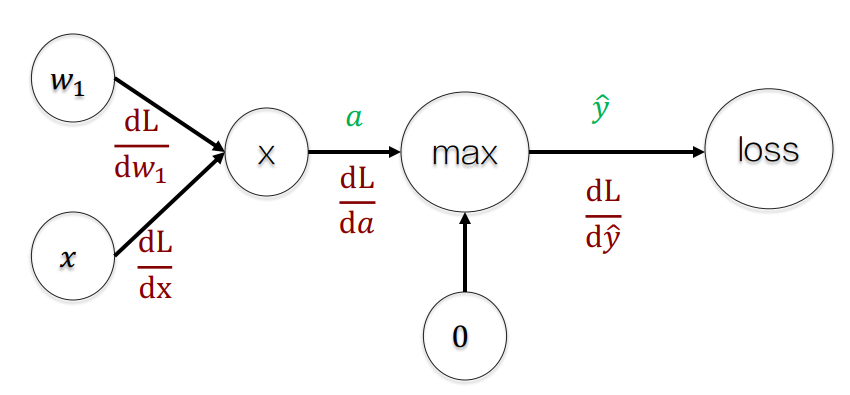
\includegraphics[width=6cm]{Capture.png}
\centering
\caption{1D example (CS 131 lecture slide 20-10)}
\end{figure}
 \\
In order to demonstrate backprop, we will use a 1-d neural network as an example. In this case, $a = wx$, and $\hat{y} =$ max($0,a$). Our goal is to calculate $dL/dW$. Using the chain rule, we can see that $dL/dw_1 = dL/da * da/dw_1$, and $dL/da = dL/d\hat{y} * d\hat{y}/da$. We can then apply the chain rule to solve.

\subsection{Rules for Calculating Gradients}

There are some general rules that can help when calculating gradients of input features. If the operation is addition, then the gradients of the input features are distributed in that $\frac{dL}{dx_i} = \frac{dL}{dy}$ for all input features $x_i$. If the operation is multiplication, then each gradient will be proportional to the values of the other input features. For example, if there are two input features $w$ and $x$, then $\frac{dL}{dw} = x\frac{dL}{dy}$ and $\frac{dL}{dx} = w\frac{dL}{dy}$. If the operation is a maximum function, like $y = $ max$(x, w)$, then $\frac{dL}{dw} = \frac{dL}{dy}$ if $w \geq x$ and 0 otherwise; $\frac{dL}{dx} = \frac{dL}{dy}$ if $x \geq w$ and 0 otherwise. If the function is $y = e^x$, then $\frac{dL}{dx} = y \frac{dL}{dy}$, since $\frac{dy}{dx} = e^x$.



\section{Convolutional Neural Networks}

Convolutional neural networks are a type of deep learning models that are often used for object recognition and classification. At a high level, CNNs start with an original image, and convolve it with multiple filters. The parameters for convolution are also chosen via backpropagation, ensuring that we do not have to hand-choose features.

Convolutional neural networks can be broken down into 3 steps
1) Convolution, 2) Non Linearity,
3) Pooling

\subsection{Convolution:} We use convolution in this step as a means to extract features from the original input image. A CNN learns the values of the filters or kernels during the training process. Typically we use 1 2D convolution layer on black and white images; however, if you wanted to extract features from a color image you can use 3 2D convolution layers (one for each channel).

The size of the convolved feature is controlled by three parameters: depth, stride, and zero-padding that we need to decide before the convolution step is performed. Depth corresponds to the number of filters we use for the convolution operation. Stride is the number of pixels by which we slide our filter matrix over the input matrix. We use zero-padding to apply the filter to bordering elements of our input image matrix. Zero padding also allows us to control the size of the feature maps. 

Introduce Non-Linearity (ReLu Function):
After every convolution, the ReLu function is applied to introduce non-linearity in our model (because most real-world data we would want our ConvNet to learn would be non-linear.) ReLU stands for Rectified Linear Unit and its output is given by the following:
\begin{figure}[h]
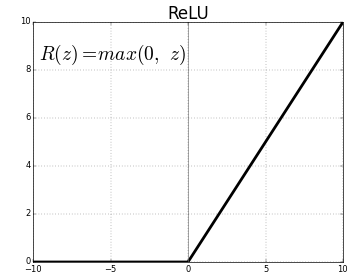
\includegraphics[width=6cm]{relu.png}
\centering
\caption{The ReLU function. (Kanchan Sarkar, Medium))}
\end{figure}

Other non-linear functions that can be applied to the convolved images include the sigmoid and tanh function; however, the ReLu function tends to give the best results.

\subsection{Pooling}
Modern convolutional neural networks incorporate pooling layers -- layers in the neural network that downsize the dimensionality but retain the most important information. This works by defining a spatial neighborhood, such as a 2x2 window, and then taking different data from the neighborhood depending upon the pooling algorithm. One example of this sort of pooling is MaxPool, where the max value in the window is the value that is retained. There are other pooling algorithms, such as AveragePool and SumPool, where the average is taken and the sum of the window is taken.

\begin{figure}[h]
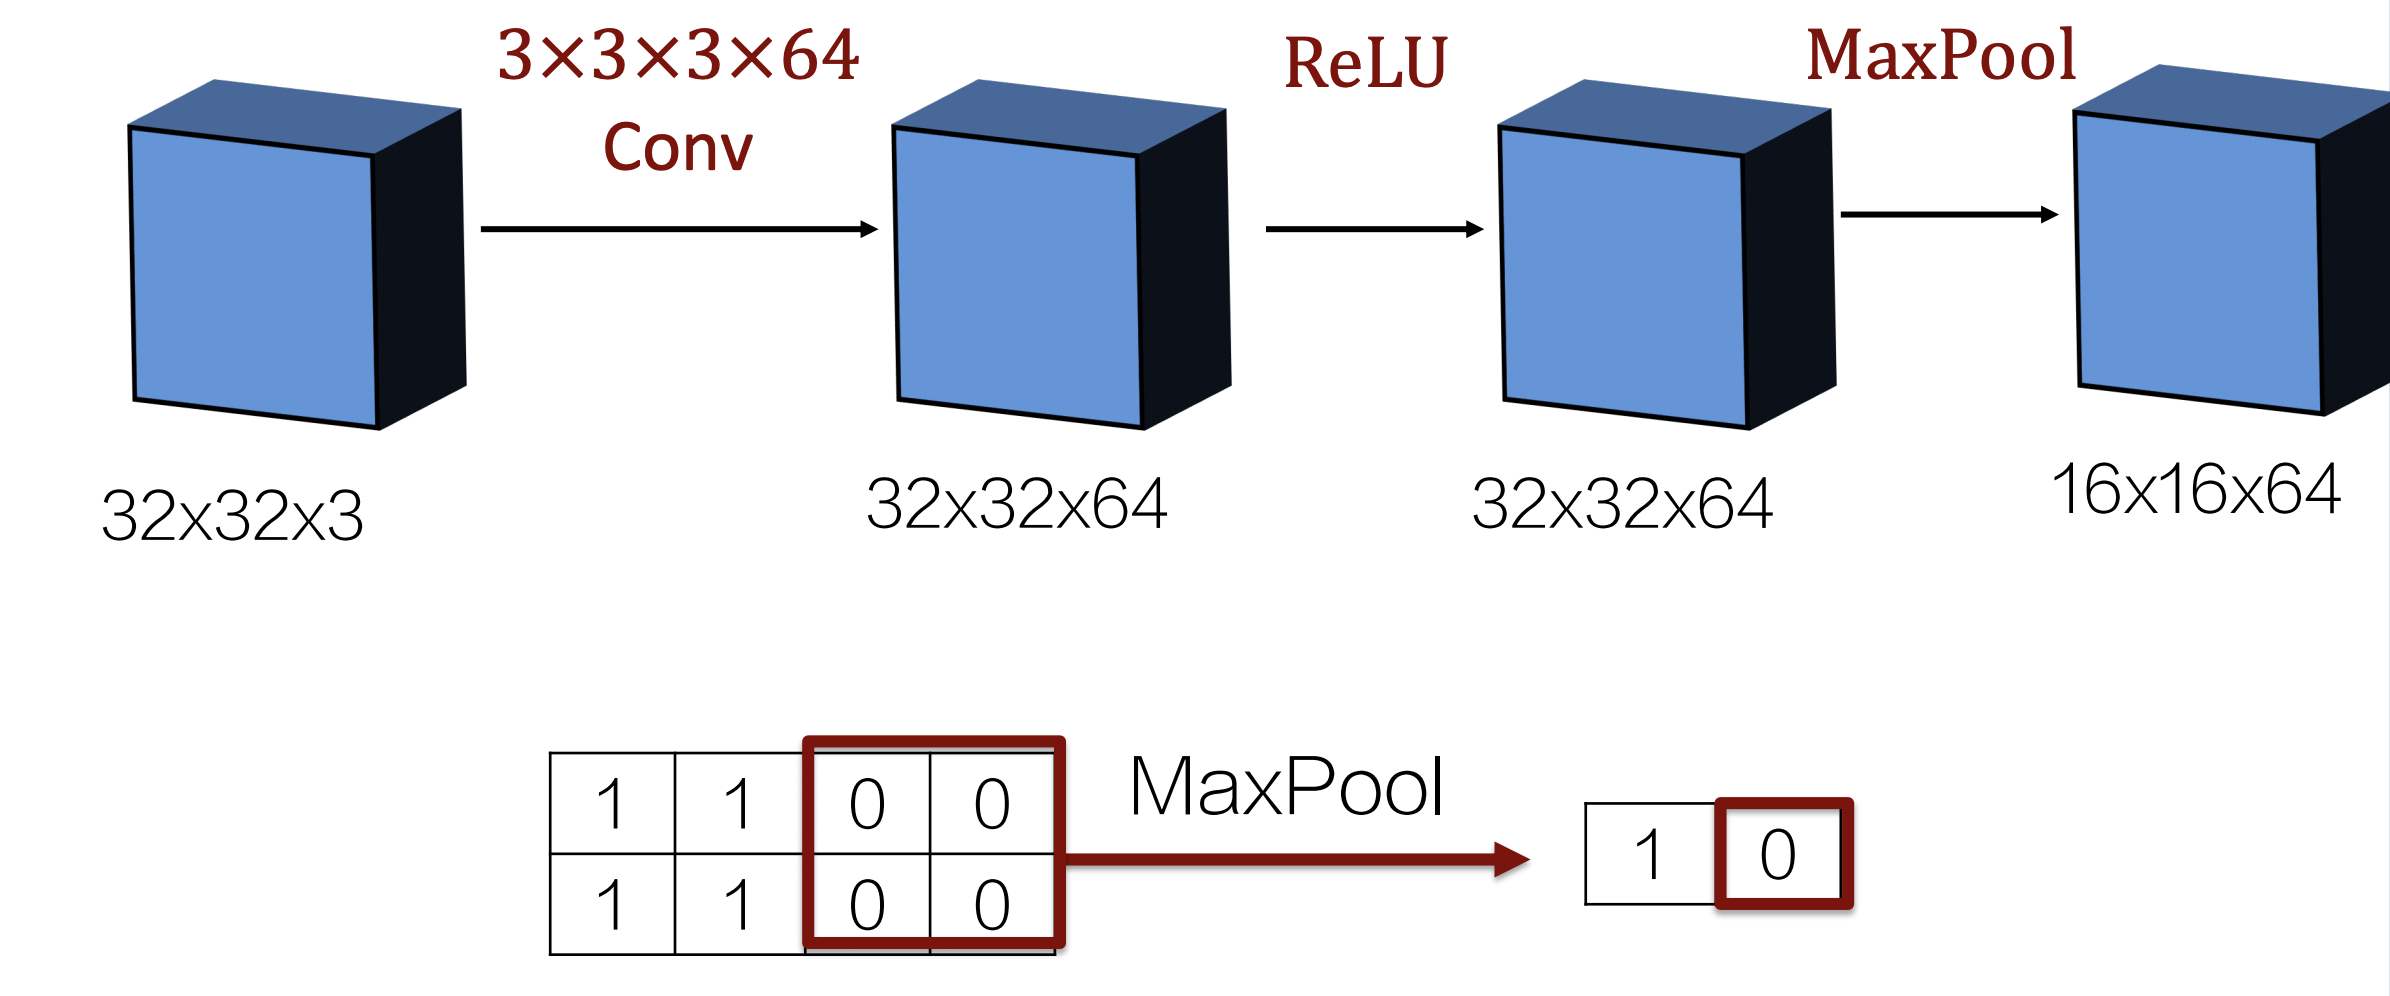
\includegraphics[width=6cm]{maxpooling.png}
\centering
\caption{Max pooling reduces dimensionality by a factor of 2. (CS 131 lecture slide 20-38)}
\end{figure}
 
\subsection{Architecture}
These different layers can be stacked, feeding the input of one layer into the other in order to help improve output quality. These layers extract relevant information, and then classify.

\begin{figure}[h]
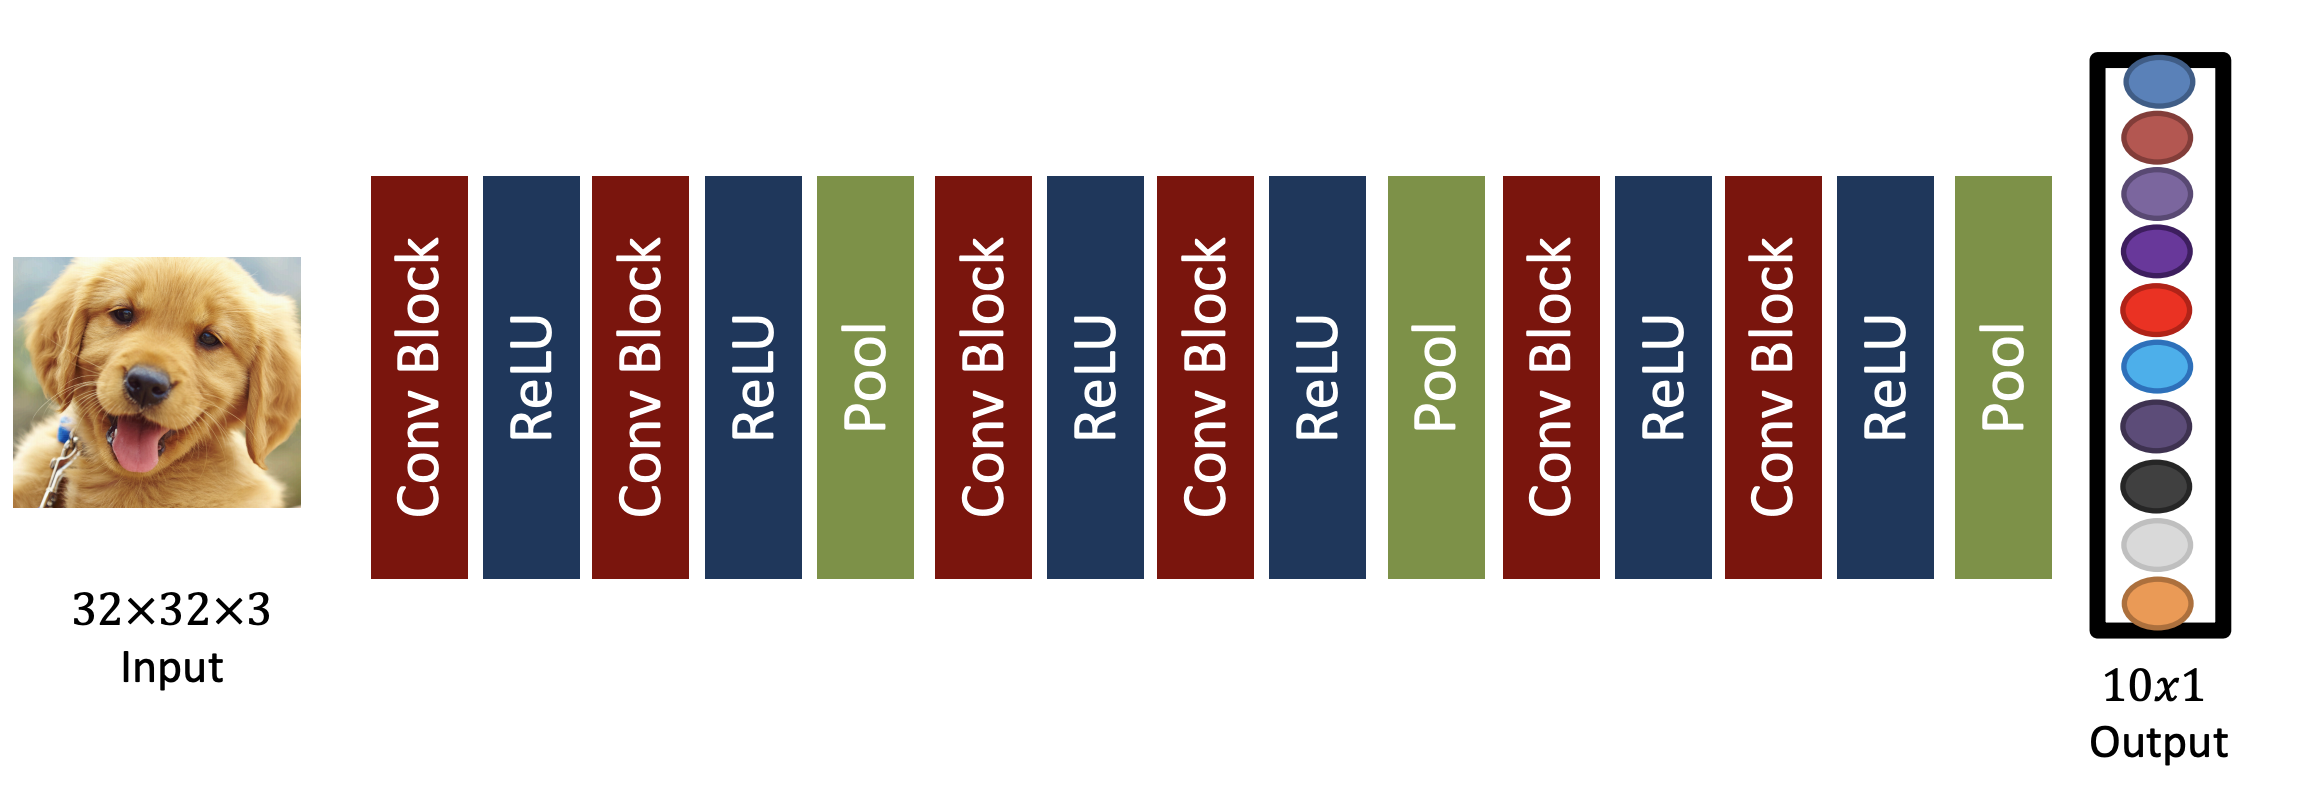
\includegraphics[width=6cm]{structure.png}
\centering
\caption{CNN Architecture (CS 131 lecture slide 20-41)}
\end{figure}

This basic structure can be expanded -- consider GoogLeNet, a CNN with an Inception layer, a hand-designed network within a network. 

\begin{figure}[h]
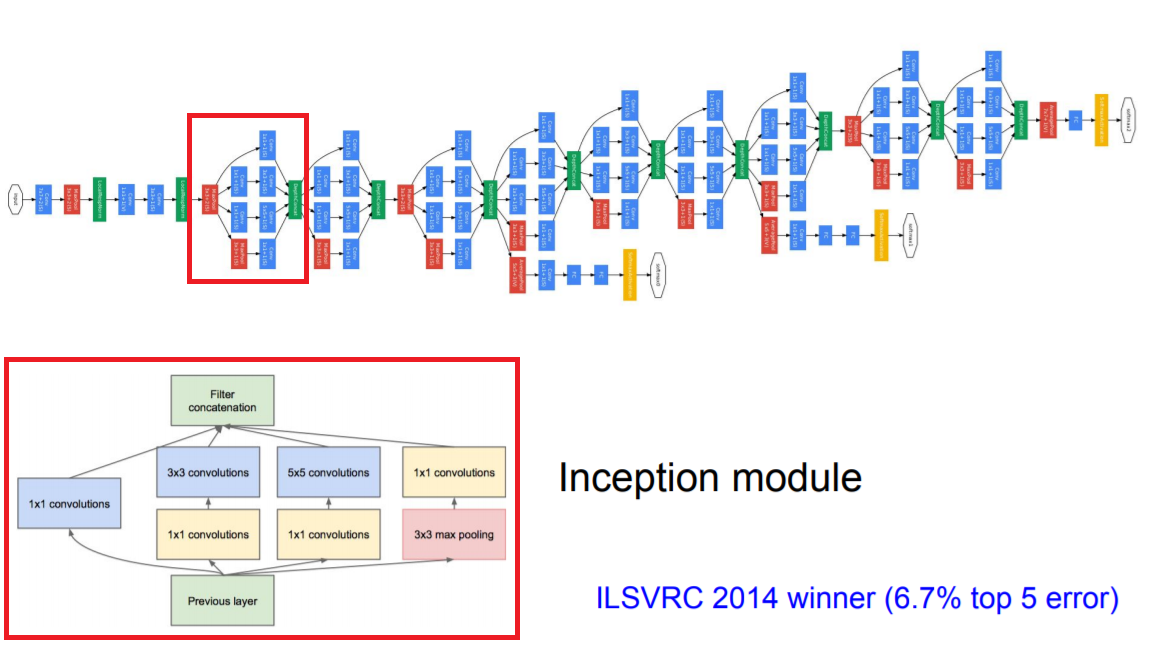
\includegraphics[width=6cm]{Inception.png}
\centering
\caption{GoogLeNet architecture and Inception module. (CS 131 lecture slide 19-101)}
\end{figure}

However, this layering process comes with a drawback. Convolutional neural networks are not shift-invariant, due to the pooling layer -- minor shifts in the image can result in dramatically different classification outputs. (Best demonstrated here: https://richzhang.github.io/antialiased-cnns/). One potential solution would be the BlurPool algorithm, where the window is blurred and shifted before MaxPool is ran, resulting in better outcomes. However, this does not solve the shift-invariance problem, so results may still be unpredictable.
 
\section{Conclusion}
While CNNs meet the basic architecture described above, there are still many variations between different networks. CNNs can differ by the amount of layers or values of the hyperparameters used. If you are interested in learning more about different CNNs, read more on  GoogLeNet, VGGNet, or ZF Net.

% References
\small
\bibliographystyle{plain}
\bibliography{bibliography}
\end{document}
